\chapter{Main Concepts}
\label{ch:concepts}
% Describe your own work (how you reached your goal) and take care to motivate your choices. Don't just describe all the things you did – tell us why.
% Background theory and main concepts

This chapter introduces essential concepts that futher work builds on.


%------------------------------------
\section{Rooted, Labeled, and Ordered Trees}

An HTML document is a \emph{labeled rooted tree} with a defined vertex order, i.e. depth-first pre-order traversal. It has a single root vertex (an \texttt{<HTML>} element) and contains vertexes labeled from a finite set of tag names: \texttt{<P>}, \texttt{<DIV>}, \texttt{<H1>}, \texttt{<STRONG>}, etc. The labeling marks element type, which carries semantics associated with it. Unless specified otherwise, all trees we discuss in this paper are rooted, labeled and ordered.

In our paper, we use $w$ to notate a web page. A specific version of a web page, i.e. a \emph{snapshot}, is marked with an subscript as $w_i$. The notation $w_1$ and $w_2$ means, that we have two snapshots of the same web page $w$, and the second $w_2$ is a newer version of $w_1$. These snapshots might be equal or slighly different.

As an example, consider the Figure~\ref{fig:amazon-books-html}, representing the rendered HTML of a book listings page, and the Figure~\ref{fig:amazon-books-tree}, displaying the tree representation of the same HTML document. It is a labeled ordered rooted tree: there is a single root element \texttt{<HTML>}, every child node has a fixed order, and labels are from a finite HTML tag set.

Most elements at the leaves of an HTML tree are text nodes (marked in italic in Figure~\ref{fig:amazon-books-tree}). In our algorithm, we are primarily interested in the structure of the tree, but not the content of the nodes. Thus, we treat all HTML text elements as of type \texttt{TEXT}. Although, as described in Section~\ref{sec:future-work}, taking into account the content patterns might be an interesting extension point for our algorithm.

Two HTML documents $w_1$ and $w_2$ are \emph{isomorphic}, if they have identical tree structure and labels. In other words, there is a mapping between each vertex in both trees that respects labels and order. A tree \emph{alignment} is a mapping of nodes from one tree to another that respects both the hierarchical relation between nodes and the order between sibling nodes. No node can appear more than once in a mapping. A \emph{maximum alignment} includes a mapping with maximum pairs. A \emph{partial alignment} does not include maximum pairs.

We use a concept of a \emph{distinguished node} in a tree $w$ (noted $d(w)$) to point to a specific vertex in this tree, that contains the textual information of interest, e.g. a title of a movie. We assume this information is important and will remain during web page updates.


%------------
\section{XML Standards}

In our work, we extensively refer to a number of World Wide Web Consortium (W3C) standards. We briefly introduce them below.

\emph{XML} (Extensible Markup Language) is a markup language that encodes a description of the document's storage layout and logical structure. \cite{w3c:xml}

\emph{DOM} (The Document Object Model) is an application programming interface (API) for valid HTML and well-formed XML documents. It defines the logical structure of documents and the way a document is accessed and manipulated. \cite{w3c:dom}

\emph{XPath} is a query language, who's primary purpose is to address the nodes of XML trees. \cite{w3c:xpath}


%---------------------
\section{Data Records}

In our work, we are particularly interested in websites that contain listings of items per single page. These data objects typically are records from some database and displayed within a fixed template. We call them \emph{data records}. Figure~\ref{fig:amazon-books-html} dispays a fragment of a web page containing book listings. Each book is a single data record with a number of \emph{attributes} displayed: title, picture, author, price, etc.

The process of identifying data records and extrating attribute values from a host web page is called \emph{data record mining}. Usually a set of data records are presented close to each other on a page with similar HTML tags, thus forming a contiguous \emph{data region}. As Liu et al. observe \cite{liu2009a}, a single web page can contain multiple data regions, and different data regions can have different data records. Figure~\ref{fig:method} visually explains the concepts in use.

\begin{figure}[h]
	\centering
	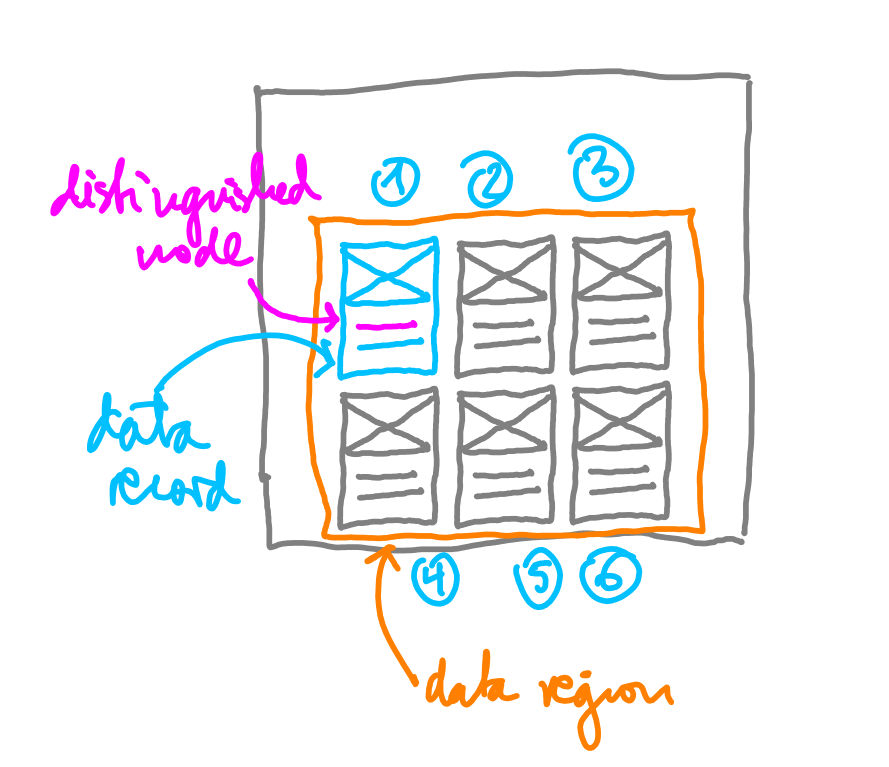
\includegraphics[width=0.5\linewidth]{figures/method}
	\caption{Elements of a data record.}
	\label{fig:method}
\end{figure}

Although data region can contain a single data record, in our work, we focus on the case with at least two data records per region.


%---------------------------
\section{Tree-Edit Distance}

In our work, we are interested in structural update to a web page. Thai \cite{Tai:1979:TCP:322139.322143} defines three operations for modeling structural change: node deletion, node insertion, and node substitution; and a certain cost is assigned to each of these operations. 

Similar to string-edit distance, \emph{tree-edit distance} between two trees $w$ and $y$ is the cost of a minimum set of operations needed to transform $w$ into $y$ \cite{zhai2005a}. Calculating a tree-edit distance between two trees is often assisted with finding a \emph{minimum-cost mapping} between two trees. 

Following the notation of Parameswaran et al. \cite{DBLP:journals/pvldb/ParameswaranDGR11}, we define a sequence $s$ of edit operations to be an \emph{edit script}. By sequentely applying the operations in $s$, we obtain a new version of the web page $w$ and denote that as $w' = s(w)$. Essentially, we can refer to an edit script as an \emph{stochastic process} $\pi$, that given a web page $w$ it creates a new version of the web page $\pi(w)$ by randomly inserting, deleting, and substituting labels. The process $\pi$ is characterized by a set of probabilities of each operation, which we define as \emph{change model}. For example, the model includes probabilities of deleting a \texttt{<P>} label or substituting \texttt{<H1>} with \texttt{<H2>}.


%----------------
\section{Web Wrapping}

The term \emph{wrapper} originates from information system integration domain \cite{Chang:2006:SWI:1159162.1159300}, where a proxy interface abstracts away the complexity of accessing a data source. We define a \emph{web wrapper} as a function that given a web page $w$ with a location of a labeled node $d(w)$, returns a set of nodes from a future version of $w$ that $d(w)$ was mapped to. To be specific, we are interested in the actual text data that is contained in mapped nodes. A \emph{successful wrapper} correctly identifies a mapped node and extracts expected information. A \emph{wrapper breaks} when it fails to locate the position of a disinguished node in a transformed web page.


% vim:wrap linebreak nolist:
